% !TEX program = tectonic
% Slides « La couche données — collecte & validation » (présentation chef, ~10 min).
% Tous les chiffres proviennent de docs/RAPPORT_QUALITE.md (généré par python -m common.quality,
% offline, cohérent avec les CSV FINAL) — références de section en commentaire sur chaque slide.
% Figures : docs/quality/*.png (générées par common.quality) + docs/slides/*.png (deck) +
% docs/sources/*.png (captures des 4 formats source).
\documentclass[11pt,aspectratio=169]{beamer}
\usetheme{default}
\usecolortheme{seagull}
\setbeamertemplate{navigation symbols}{}
\setbeamertemplate{footline}{%
  \hfill\textcolor{black!45}{\scriptsize\insertframenumber\,/\,\inserttotalframenumber}\hspace{2mm}\vspace{1.5mm}}
\usepackage[T1]{fontenc}
\usepackage{lmodern}
\usepackage[utf8]{inputenc}
\usepackage[french]{babel}
\usepackage{booktabs}
\usepackage{xcolor}
\usepackage{graphicx}
\usepackage{fancyvrb}
\usepackage{amssymb}
\usepackage{textcomp}
\usepackage{array}
\usepackage{newunicodechar}
\usepackage{tikz}
\usetikzlibrary{arrows.meta,positioning,calc}

% Caractères Unicode → commandes (fontes T1)
\newunicodechar{→}{\ensuremath{\rightarrow}}
\newunicodechar{—}{\textemdash}
\newunicodechar{–}{\textendash}
\newunicodechar{…}{\ldots}
\newunicodechar{·}{\textperiodcentered}
\newunicodechar{≈}{\ensuremath{\approx}}
\newunicodechar{×}{\ensuremath{\times}}
\newunicodechar{≤}{\ensuremath{\leq}}
\newunicodechar{≥}{\ensuremath{\geq}}
\newunicodechar{−}{\ensuremath{-}}
\newunicodechar{✓}{\checkmark}
\newunicodechar{✗}{\ensuremath{\times}}
\newunicodechar{°}{\textdegree}
\newunicodechar{§}{\S}
\newunicodechar{«}{\og}
\newunicodechar{»}{\fg{}}

% Code couleur des 4 voies (repris dans toutes les figures)
\definecolor{helec}{HTML}{3B6EA5}   % House électronique
\definecolor{hocr}{HTML}{A9C5E2}    % House OCR
\definecolor{selec}{HTML}{8E44AD}   % Sénat électronique
\definecolor{socr}{HTML}{CFAEDE}    % Sénat OCR
\definecolor{okgreen}{HTML}{2E8B57}
\definecolor{alertred}{HTML}{C0392B}
\definecolor{warnorange}{HTML}{E67E22}

\setbeamercolor{frametitle}{fg=helec,bg=white}
\setbeamerfont{frametitle}{series=\bfseries,size=\large}
\setbeamercolor{title}{fg=helec}
\setbeamercolor{structure}{fg=helec}

% Tuile chiffre-clé : \tuile{couleur}{gros chiffre}{légende}
\newcommand{\tuile}[3]{%
  \begin{minipage}[t]{0.23\textwidth}\centering
    \colorbox{#1}{\parbox[c][21mm][c]{\dimexpr\linewidth-8pt}{\centering
      {\color{white}\Large\textbf{#2}}\\[0.6mm]
      {\color{white}\footnotesize #3}}}
  \end{minipage}}

% Badge coloré une ligne
\newcommand{\badge}[2]{\colorbox{#1}{\textcolor{white}{\footnotesize\textbf{#2}}}}
\newcommand{\badgel}[2]{\colorbox{#1}{\textcolor{black!80}{\footnotesize\textbf{#2}}}}

\title{La couche données — collecte \& validation}
\subtitle{Transactions boursières du Congrès américain · Chambre \& Sénat · 2014--2026}
\author{Alice Lemaire}
\date{Juillet 2026}

\begin{document}

% ───────────── S1 · Titre ─────────────
% Chiffres : RAPPORT_QUALITE §Résumé (169 000 ; 367+78=445) ; §1 (4 sous-corpus)
\begin{frame}
  \vspace{6mm}
  {\color{helec}\LARGE\textbf{La couche données — collecte \& validation}}\\[1.5mm]
  {\large Transactions boursières du Congrès américain · Chambre \& Sénat · 2014--2026}\\[1mm]
  {\color{black!55}\small Alice Lemaire · juillet 2026}
  \vspace{9mm}

  \centering
  \tuile{helec}{169\,000}{transactions uniques}\hfill
  \tuile{selec}{13 ans}{2014 → 2026}\hfill
  \tuile{okgreen}{445}{élus identifiés\\(367 Chambre + 78 Sénat)}\hfill
  \tuile{warnorange}{4 voies}{2 chambres × 2 formats\\(électronique / papier scanné)}
\end{frame}

% ───────────── S2 · La règle du jeu ─────────────
% Chiffres : STOCK Act 45 j (loi) ; délai médian 27/24 j (§3) ; 8 252 PTR (§1)
\begin{frame}{La règle du jeu : le STOCK Act (2012)}
  \begin{columns}[T]
    \begin{column}{0.52\textwidth}
      \centering
      \begin{tikzpicture}[
        box/.style={draw=none, rounded corners=2pt, fill=black!6, minimum height=8.5mm,
                    align=center, font=\footnotesize, inner xsep=2.5mm},
        arr/.style={-{Latex[length=2.2mm]}, thick, black!55}]
        \node[box] (t) {un élu\\\textbf{trade}};
        \node[box, right=11mm of t] (p) {dépôt d'un\\\textbf{PTR}};
        \node[box, right=11mm of p] (w) {\textbf{publication}\\en ligne};
        \draw[arr] (t) -- node[above, font=\scriptsize\bfseries, color=alertred] {≤ 45 j} (p);
        \draw[arr] (p) -- (w);
      \end{tikzpicture}

      \vspace{5mm}
      \begin{minipage}{0.95\linewidth}\footnotesize
        \colorbox{helec}{\textcolor{white}{\textbf{Chambre}}} disclosures-clerk.house.gov\\[0.5mm]
        {\color{black!60}\scriptsize PTR = \emph{Periodic Transaction Report} — \textbf{8\,252} PTR officiels sur 13 ans}\\[2.5mm]
        \colorbox{selec}{\textcolor{white}{\textbf{Sénat}}} efdsearch.senate.gov (eFD)\\[0.5mm]
        {\color{black!60}\scriptsize déclarations électroniques + scans papier}
      \end{minipage}
    \end{column}
    \begin{column}{0.46\textwidth}
      \centering
      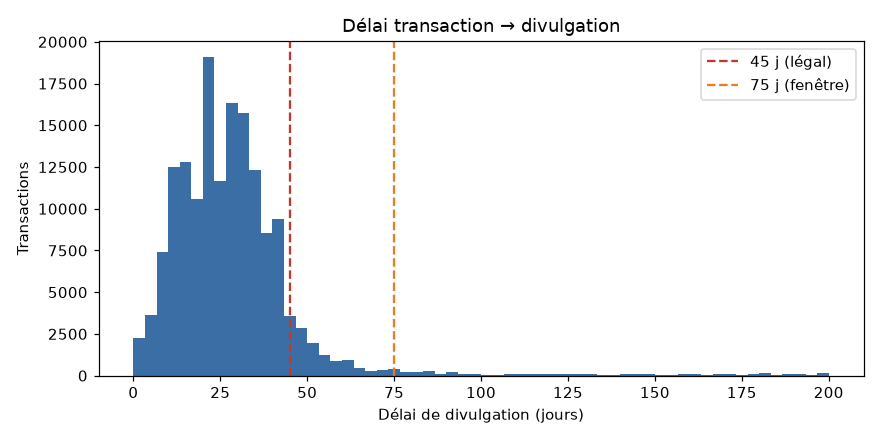
\includegraphics[width=\linewidth]{quality/delai_divulgation.png}\\[1mm]
      \badge{okgreen}{délai médian réel : 27 j Chambre · 24 j Sénat}
    \end{column}
  \end{columns}
\end{frame}

% ───────────── S3 · Les 4 visages ─────────────
% Volumes : §1 « quatre sous-corpus » (58 728 / 93 261 / 13 026 / 3 985)
\begin{frame}{Une même loi, quatre visages de la donnée}
  \centering
  \begin{minipage}[t]{0.40\textwidth}\centering
    \fcolorbox{helec}{white}{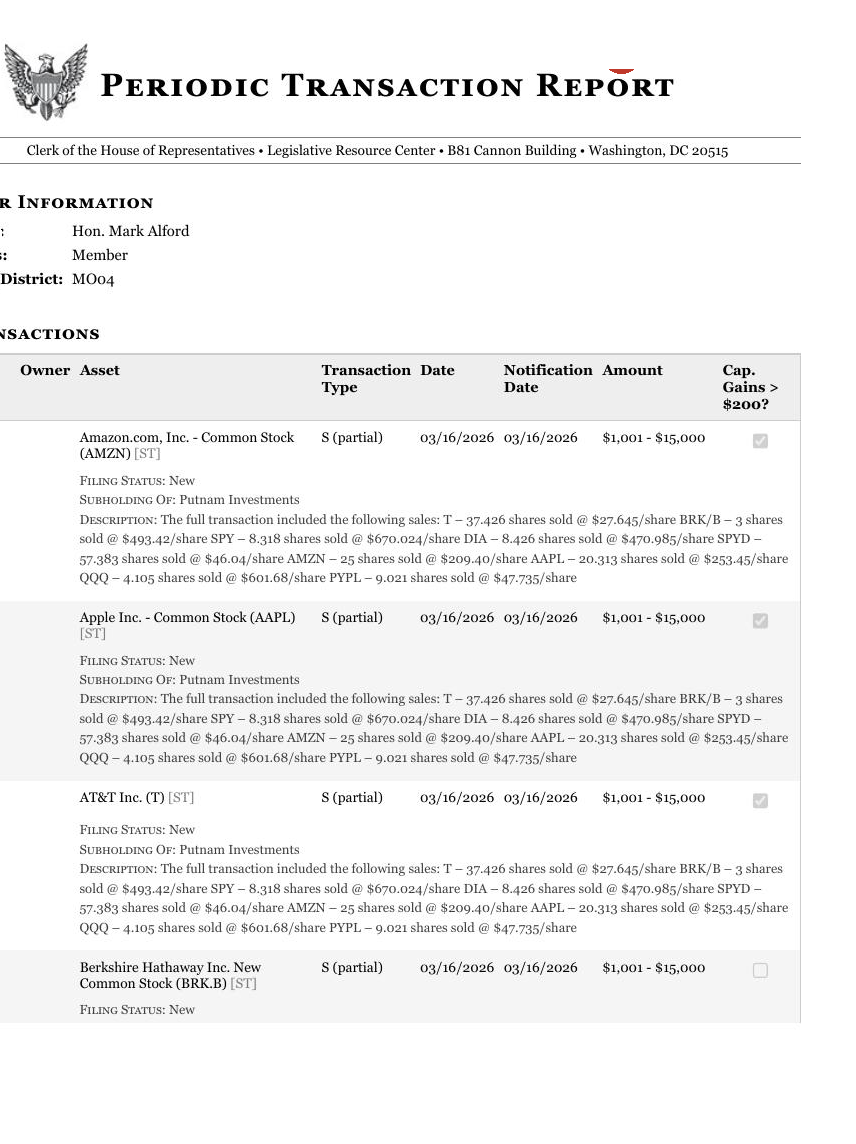
\includegraphics[height=25mm]{sources/house_digital.png}}\\[0.6mm]
    \badge{helec}{Chambre électronique — 58\,728}
  \end{minipage}\hspace{6mm}
  \begin{minipage}[t]{0.40\textwidth}\centering
    \fcolorbox{hocr}{white}{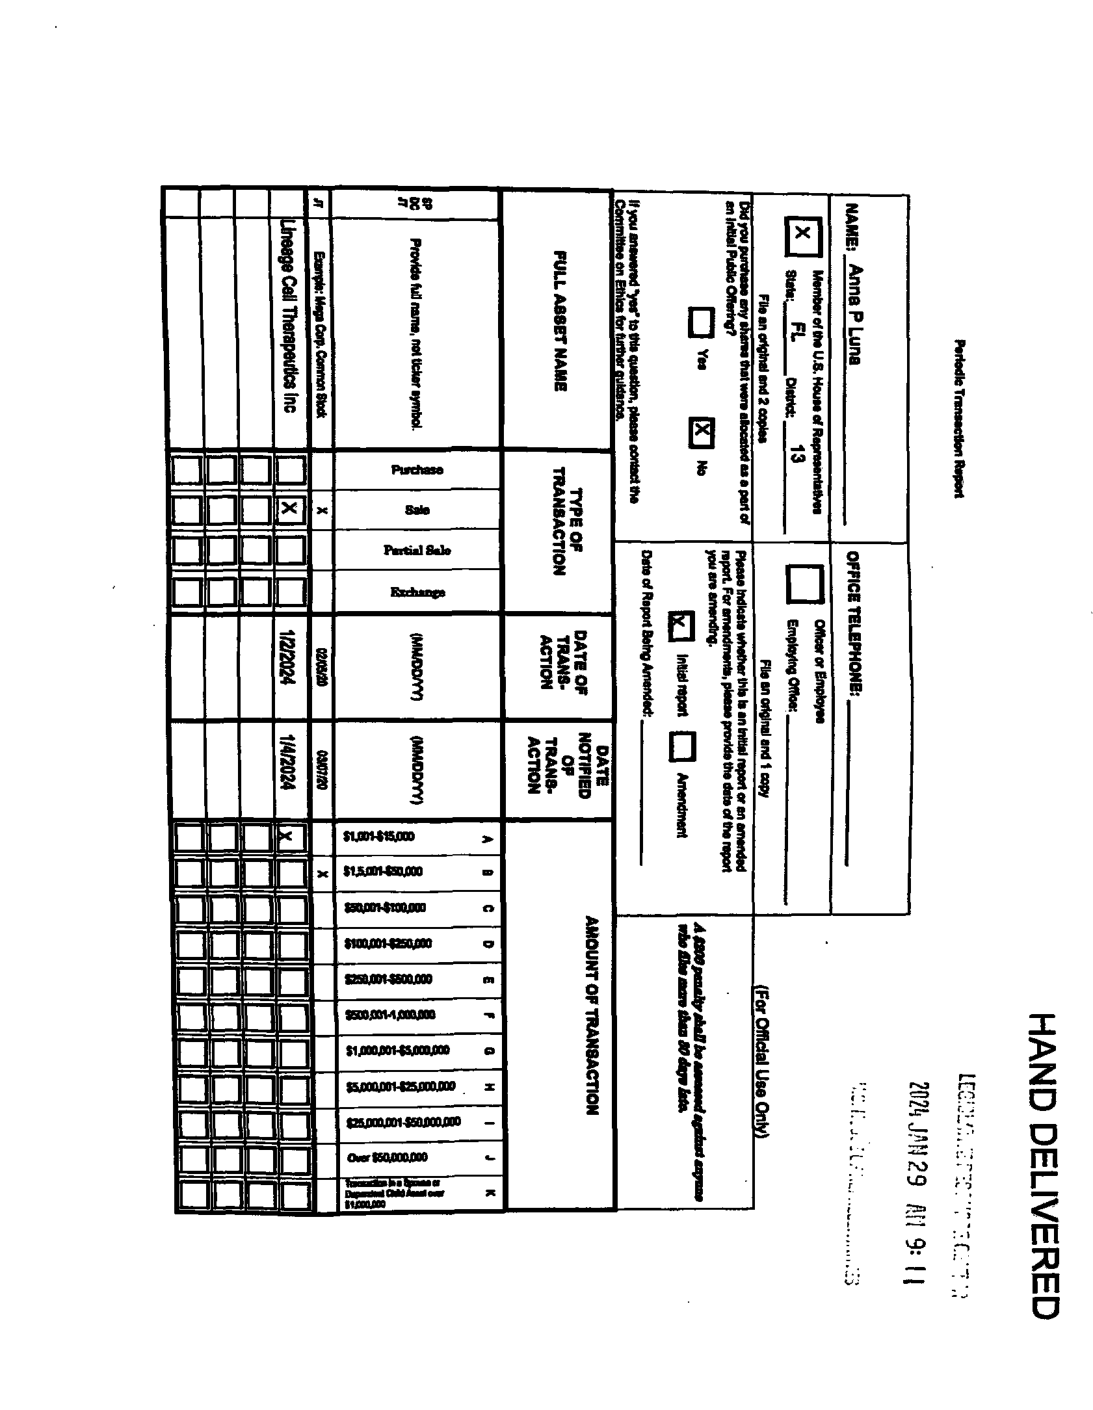
\includegraphics[height=25mm]{sources/house_ocr.png}}\\[0.6mm]
    \badgel{hocr}{Chambre scannée (OCR) — 93\,261}
  \end{minipage}

  \vspace{3.5mm}
  \begin{minipage}[t]{0.40\textwidth}\centering
    \fcolorbox{selec}{white}{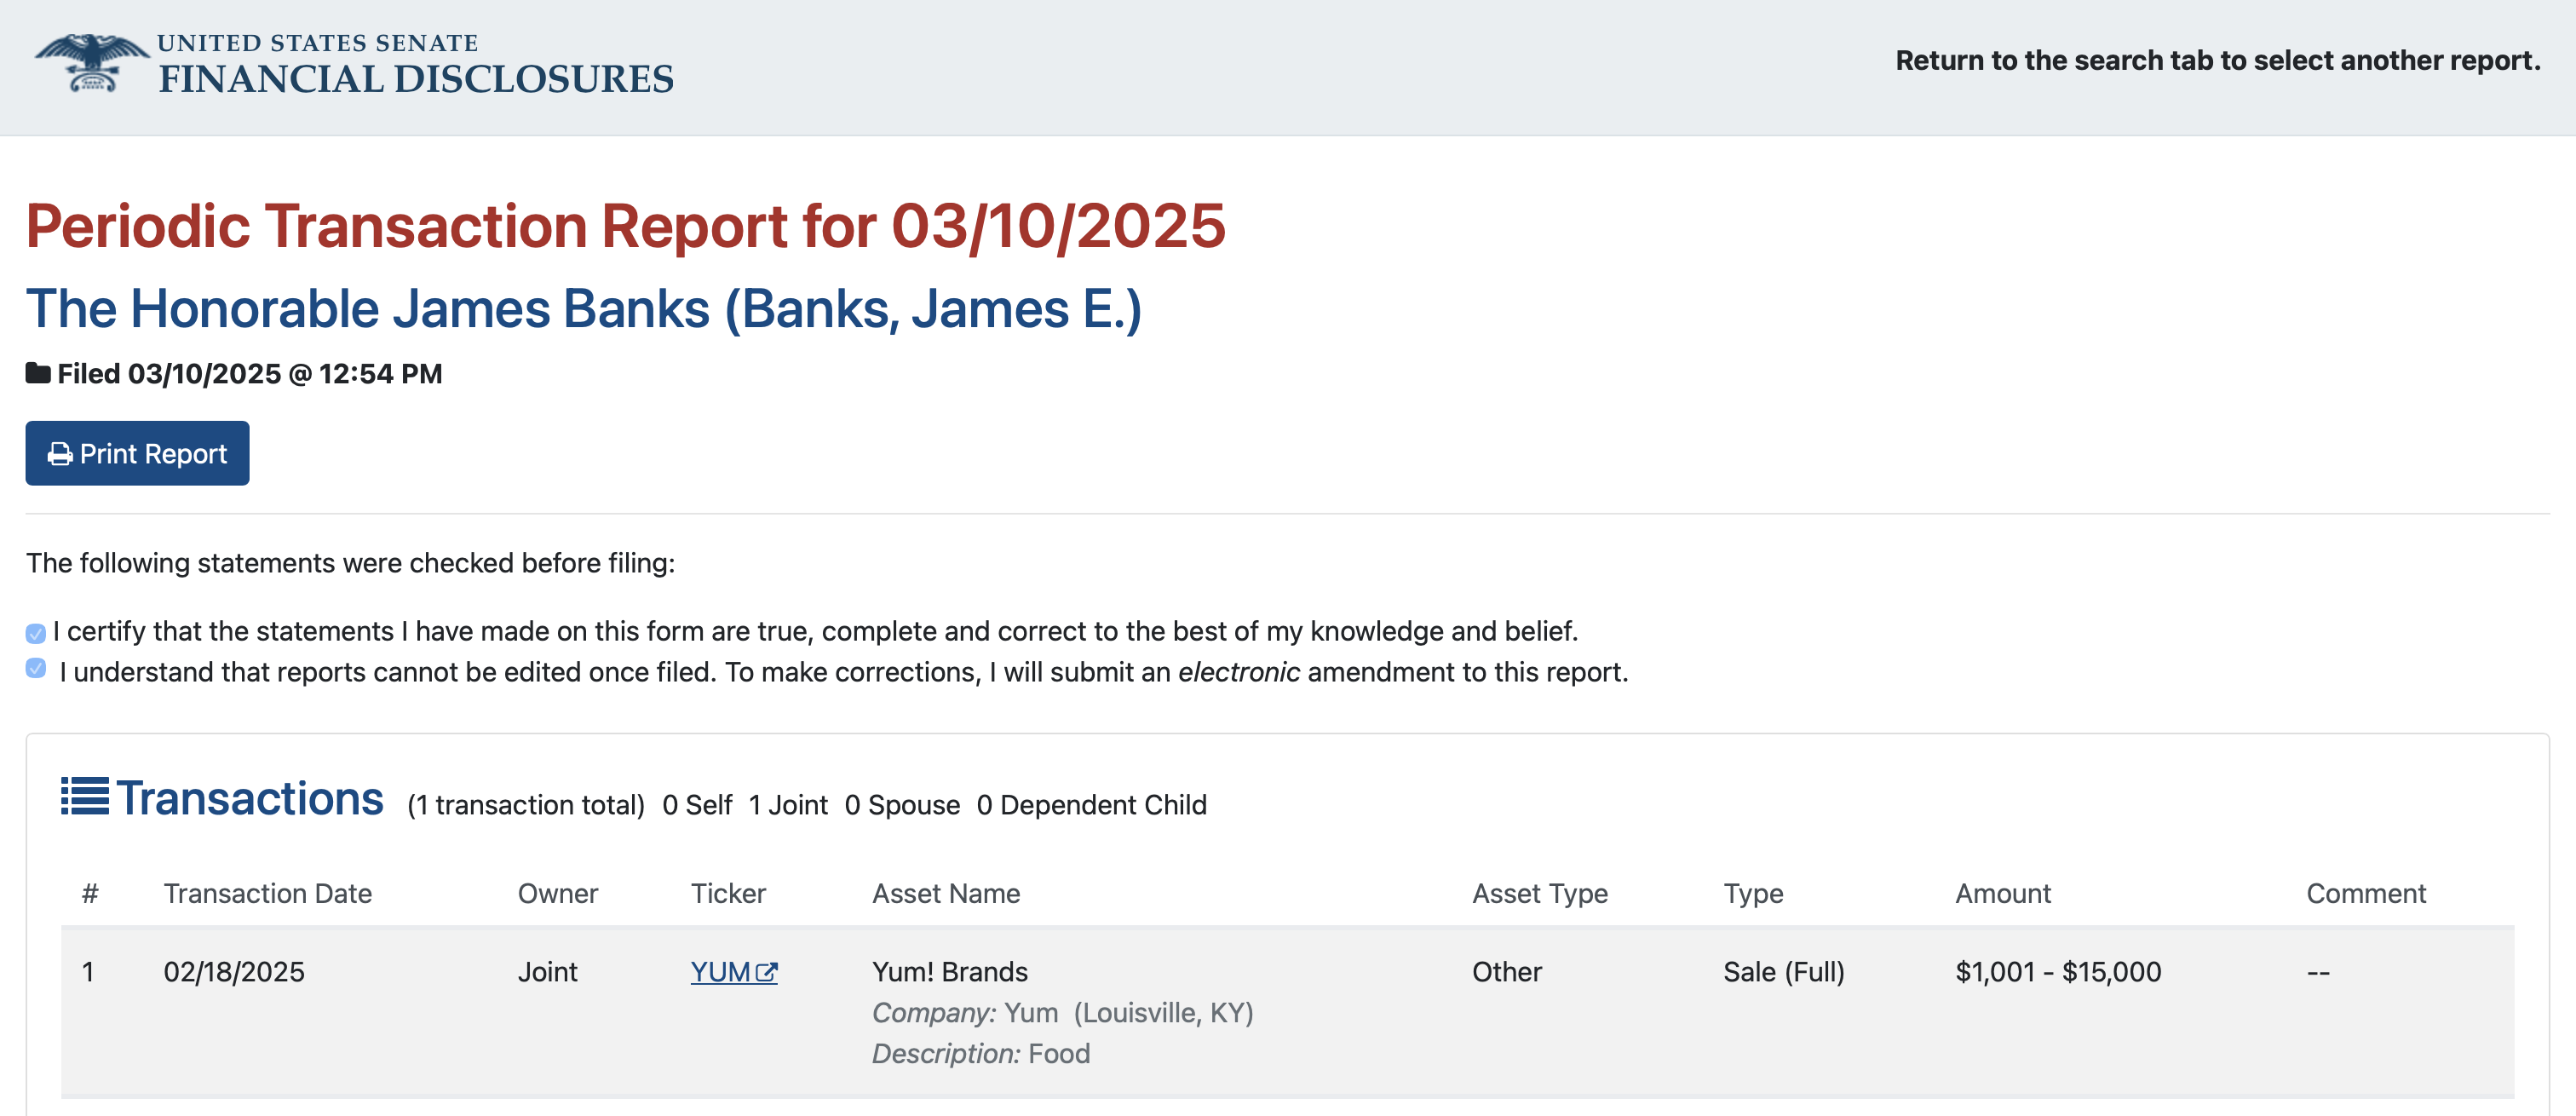
\includegraphics[height=25mm]{sources/senate_digital.png}}\\[0.6mm]
    \badge{selec}{Sénat électronique — 13\,026}
  \end{minipage}\hspace{6mm}
  \begin{minipage}[t]{0.40\textwidth}\centering
    \fcolorbox{socr}{white}{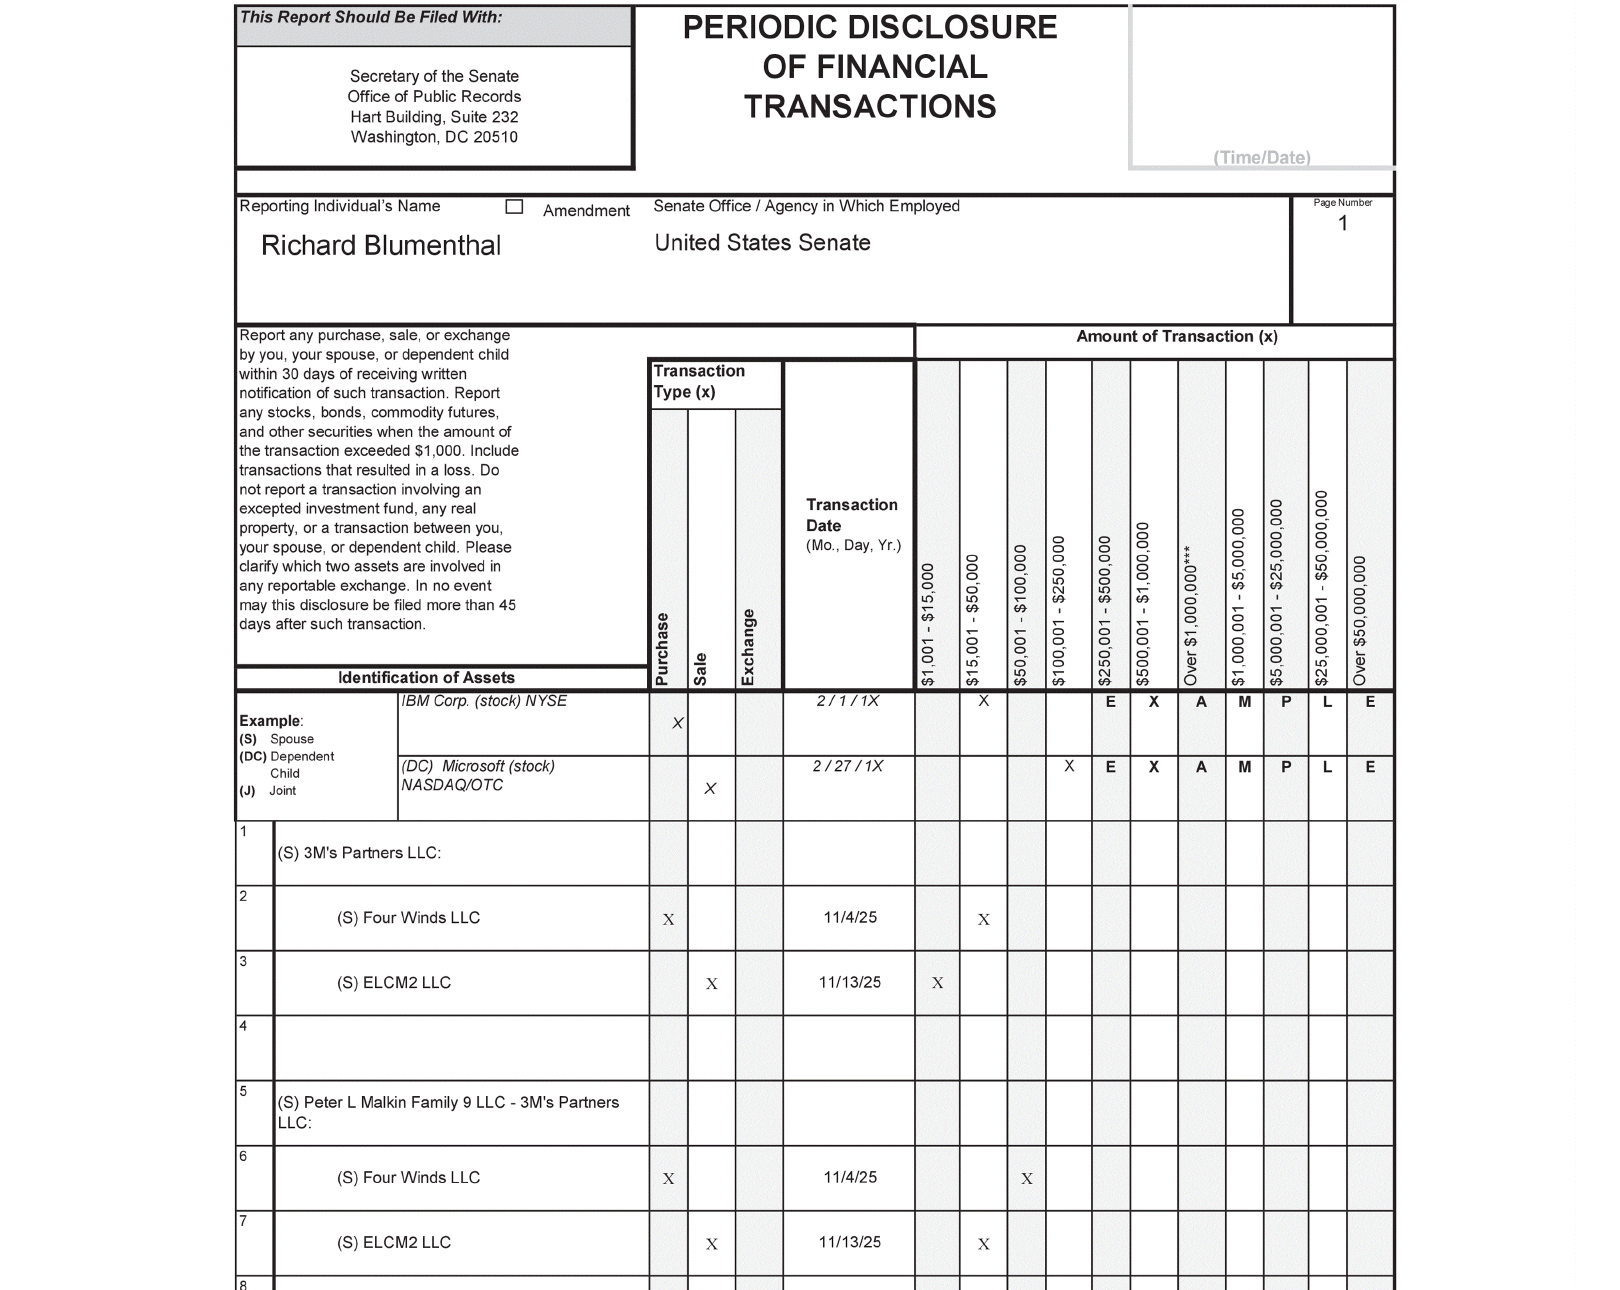
\includegraphics[height=25mm]{sources/senate_ocr.png}}\\[0.6mm]
    \badgel{socr}{Sénat papier (OCR) — 3\,985}
  \end{minipage}

  \vspace{2.5mm}
  {\scriptsize\color{black!60} du formulaire web propre… au scan tourné à 90° déposé à la main
  (tampon \emph{HAND DELIVERED})}
\end{frame}

% ───────────── S4 · Schéma maître ─────────────
% Chiffres : §1 réconciliation (170 920 / 1 920 / 169 000), §7 (134 464×36), golden 368 (§1)
\begin{frame}{Quatre voies, une table}
  \centering
  \resizebox{\textwidth}{!}{%
  \begin{tikzpicture}[
    src/.style={draw=none, rounded corners=2pt, minimum width=4.7cm, minimum height=1.02cm,
                align=center, font=\footnotesize},
    big/.style={draw=black!25, fill=black!4, rounded corners=3pt, minimum width=2.7cm,
                minimum height=1.7cm, align=center, font=\footnotesize},
    lbl/.style={font=\scriptsize, color=black!60, align=center},
    arr/.style={-{Latex[length=2.4mm]}, thick, black!50}]
    \node[src, fill=helec, text=white] (he) {\textbf{Chambre électronique}\\PDF structurés — \textbf{58\,728}};
    \node[src, fill=hocr, below=3mm of he] (ho) {\textbf{Chambre scans → OCR}\\papier — \textbf{93\,261}};
    \node[src, fill=selec, text=white, below=3mm of ho] (se) {\textbf{Sénat électronique}\\eFD web — \textbf{13\,026}};
    \node[src, fill=socr, below=3mm of se] (so) {\textbf{Sénat papier → OCR}\\images — \textbf{3\,985}};
    \node[big, minimum height=2.4cm] (tronc) at ($(ho.east)!0.5!(se.east)+(2.6,0)$)
      {\textbf{Tronc commun}\\[0.5mm]identité · ticker\\montant · secteur};
    \draw[arr] (he.east) -- (tronc.west);
    \draw[arr] (ho.east) -- (tronc.west);
    \draw[arr] (se.east) -- (tronc.west);
    \draw[arr] (so.east) -- (tronc.west);
    \node[big, right=8mm of tronc] (raw) {\textbf{170\,920}\\lignes brutes};
    \node[big, right=13mm of raw] (uni) {\textbf{169\,000}\\transactions\\uniques};
    \node[big, right=13mm of uni, draw=helec, fill=helec!10] (bt)
      {\textbf{134\,464}\\lignes backtest\\× 36 colonnes};
    \draw[arr] (tronc) -- (raw);
    \draw[arr] (raw) -- node[above, font=\scriptsize, align=center] {dédup\\\textbf{−1\,920}} (uni);
    \draw[arr] (uni) -- node[above, font=\scriptsize, align=center] {entonnoir\\\textbf{A→D}} (bt);
    \node[lbl, below=2.5mm of uni] {golden : \textbf{368 tables figées} (SHA-256)\\+ validation externe (Quiver, stock-watchers)};
  \end{tikzpicture}}
\end{frame}

% ───────────── S5 · Acquisition Chambre ─────────────
% Chiffres : 8 252 PTR (§1) ; 5 129 PDF (find data/house/pdfs) ; ~72 ventes 2014 + 205 PTR
% hors fenêtre (house/digital.py, commentaires parse_ptr_dual / load_ptr_index)
\begin{frame}[fragile]{Acquisition Chambre : de l'index XML au PDF}
  \begin{columns}[T]
    \begin{column}{0.47\textwidth}
      \centering
      \begin{tikzpicture}[
        box/.style={draw=none, rounded corners=2pt, fill=helec!12, minimum height=7.5mm,
                    minimum width=5.4cm, align=center, font=\scriptsize},
        arr/.style={-{Latex[length=2mm]}, thick, black!50}, node distance=3.2mm]
        \node[box] (a) {index annuel \texttt{\{Y\}FD.xml} du Clerk (13 fichiers)};
        \node[box, below=of a] (b) {\texttt{FilingType='P'} → \textbf{8\,252 PTR}};
        \node[box, below=of b] (c) {téléchargement → \textbf{5\,129 PDF}};
        \node[box, below=of c, fill=hocr!45] (d) {texte incrusté ? \textbf{lisible} (parse direct)\\
              sinon \textbf{scanné} → voie OCR};
        \draw[arr] (a) -- (b); \draw[arr] (b) -- (c); \draw[arr] (c) -- (d);
      \end{tikzpicture}
    \end{column}
    \begin{column}{0.51\textwidth}
      {\scriptsize à quoi ressemble l'index (extrait réel, \texttt{2024FD.xml}) :}
\begin{Verbatim}[fontsize=\scriptsize, frame=single, rulecolor=\color{black!25}]
<Member>
  <Prefix>Hon.</Prefix>
  <Last>Allen</Last><First>Richard W.</First>
  <FilingType>P</FilingType>
  <StateDst>GA12</StateDst>
  <Year>2024</Year>
  <FilingDate>1/11/2024</FilingDate>
  <DocID>20024277</DocID>
</Member>
\end{Verbatim}
      {\scriptsize\color{black!60} \texttt{P} = PTR (les autres types : rapports annuels,
      candidatures…) — \textbf{l'index fait autorité} : 100\,\% des 8\,252 PTR traités}
    \end{column}
  \end{columns}
  \vspace{1mm}
  \colorbox{alertred!10}{\parbox{0.97\textwidth}{\footnotesize
    \textcolor{alertred}{\textbf{Pièges déjoués}} — le gabarit PDF change en 2018 :
    sans le \textbf{double parseur}, ≈\,72 ventes perdues rien qu'en 2014 (biais vendeur) ·
    \textbf{205 PTR} déposés après le 31/12 récupérés via l'index.}}
\end{frame}

% ───────────── S6 · Acquisition Sénat ─────────────
% Chiffres : 2 151 HTML cachés, 373 rapports papier (data/senate/) ; CSRF senate/digital.py
\begin{frame}{Acquisition Sénat : le portail qui résiste}
  \centering
  \begin{tikzpicture}[
    box/.style={draw=none, rounded corners=2pt, fill=selec!12, minimum height=8.5mm,
                align=center, font=\scriptsize, inner xsep=2mm},
    arr/.style={-{Latex[length=2.2mm]}, thick, black!50}]
    \node[box] (a) {efdsearch.senate.gov};
    \node[box, right=7mm of a, fill=alertred!12] (b) {agrément +\\jeton \textbf{CSRF}};
    \node[box, right=7mm of b] (c) {recherche paginée\\(type = PTR)};
    \node[box, right=7mm of c, fill=selec!25] (d) {\textbf{2\,150} pages HTML\\en cache → tables};
    \node[box, below=3mm of d, fill=socr!45] (e) {papier : \textbf{373} rapports\\en images .gif — hors barrière};
    \draw[arr] (a) -- (b); \draw[arr] (b) -- (c); \draw[arr] (c) -- (d);
    \draw[arr] (c.east) .. controls +(0.45,0) and +(-0.6,0) .. (e.west);
  \end{tikzpicture}

  \vspace{4mm}
  \begin{columns}[T]
    \begin{column}{0.33\textwidth}\centering
      \fcolorbox{selec}{white}{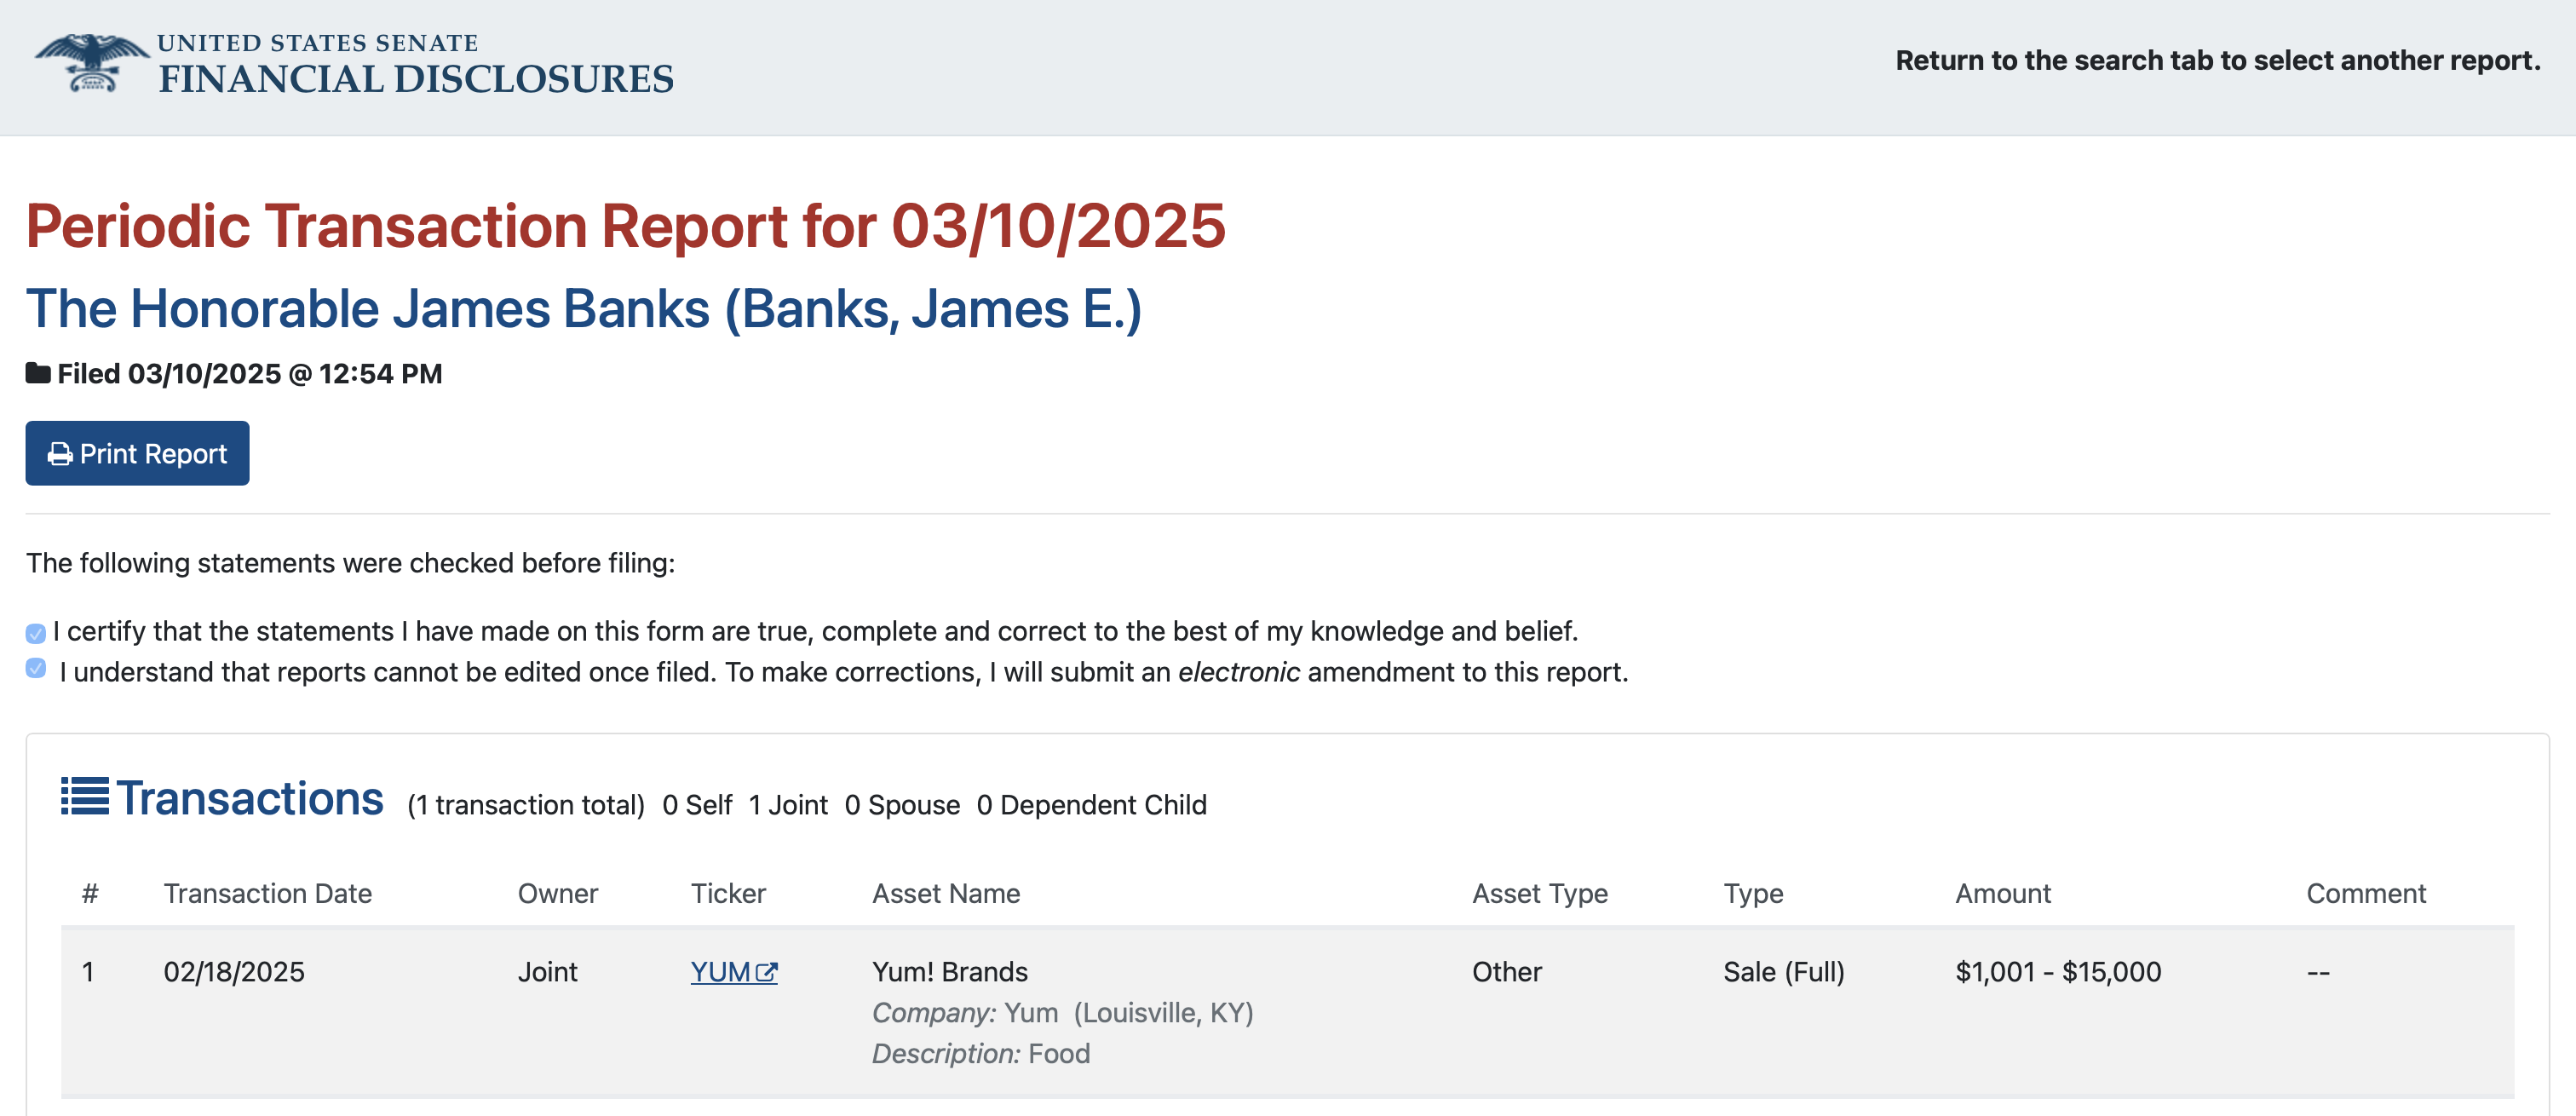
\includegraphics[height=20mm]{sources/senate_digital.png}}\\[0.5mm]
      {\scriptsize eFD électronique : table propre}
    \end{column}
    \begin{column}{0.24\textwidth}\centering
      \fcolorbox{socr}{white}{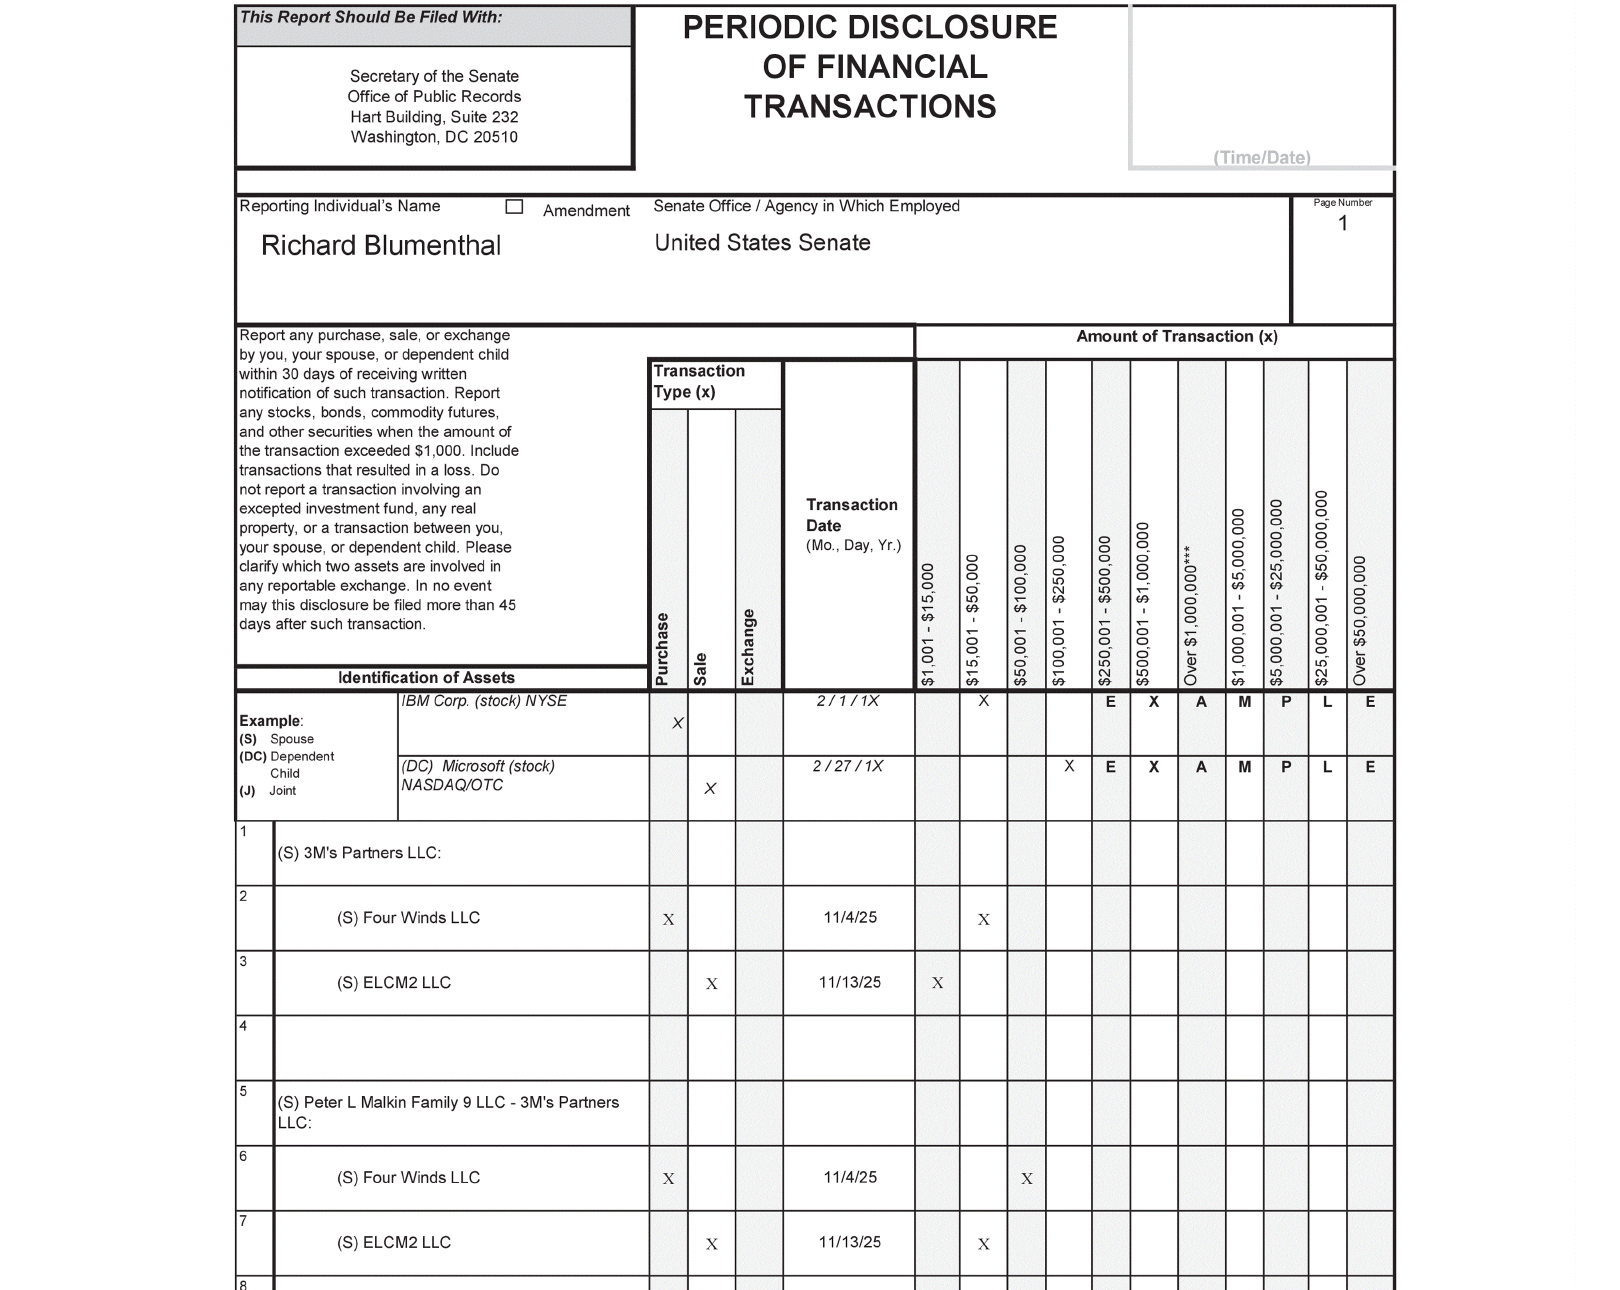
\includegraphics[height=20mm]{sources/senate_ocr.png}}\\[0.5mm]
      {\scriptsize papier : grille de cases A→L}
    \end{column}
    \begin{column}{0.38\textwidth}
      \vspace{4mm}
      \colorbox{alertred}{\parbox{0.96\linewidth}{\footnotesize\color{white}
        \textbf{Angle mort} : Quiver ne voit pas le papier Sénat
        → cette voie se valide en interne}}
    \end{column}
  \end{columns}
\end{frame}

% ───────────── S7 · La voie OCR ─────────────
% Chiffres : census 2 424 = 74+1 575+775 (_scan_census.csv) ; 582 gated (§1) ;
% corroboration par cluster 88,0/65,2/12,9 (§6.6) ; ticker LLM 46→90 % (house/ocr.py)
\begin{frame}{La voie OCR : faire lire les scans à un modèle de vision}
  \centering
  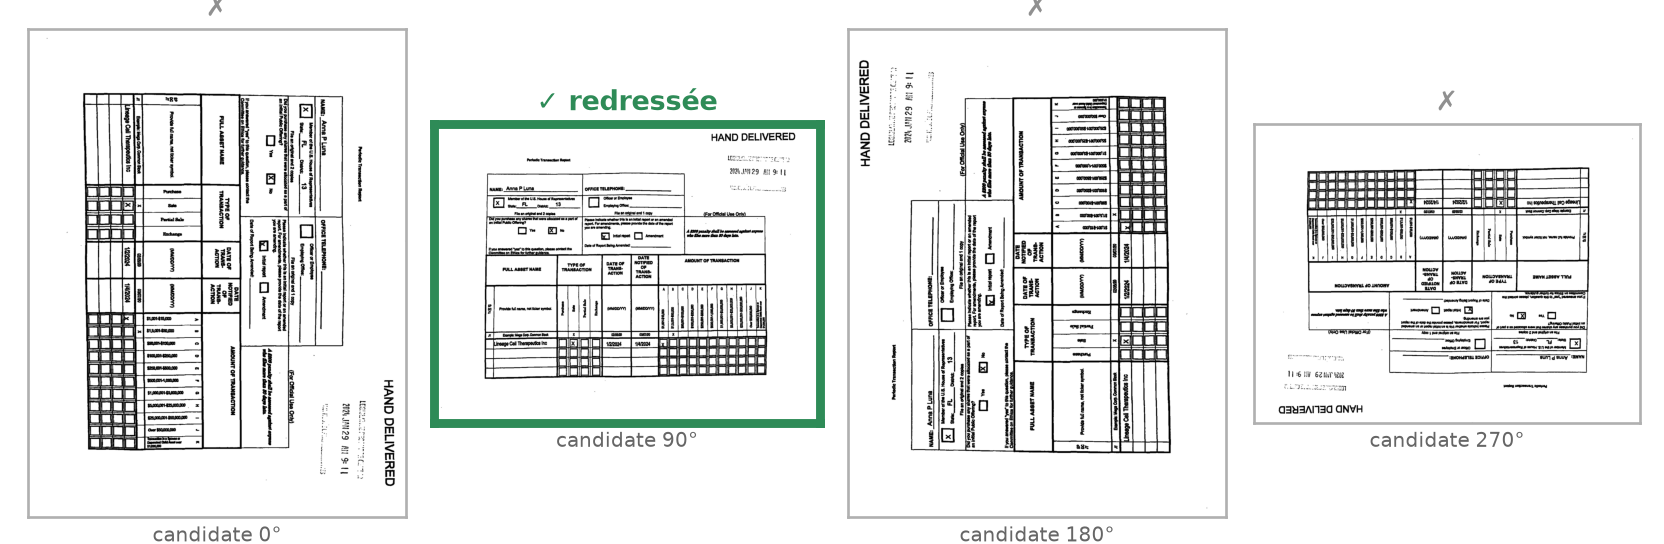
\includegraphics[width=0.78\textwidth]{slides/fig_deskew_rotations.png}

  \vspace{1.5mm}
  \begin{columns}[T]
    \begin{column}{0.48\textwidth}\footnotesize
      \textbf{1.} redresser — pré-passe Vision « choisis l'image droite »\\[0.8mm]
      \textbf{2.} classer (Vision) — census \textbf{2\,424} scans :\\
      \hspace*{3mm}{\scriptsize 74 tapés droits · 1\,575 tapés tournés · \textbf{775 manuscrits}}\\[0.8mm]
      \textbf{3.} lire — extraction structurée page à page, 200 DPI
    \end{column}
    \begin{column}{0.48\textwidth}\footnotesize
      \colorbox{black!6}{\parbox{0.97\linewidth}{\scriptsize
        \textbf{corroboration Quiver par type de scan} (§6.6) :\\
        tapé droit \textbf{88\,\%} · tapé tourné \textbf{65\,\%} ·
        manuscrit \textcolor{alertred}{\textbf{12,9\,\%}}}}\\[1mm]
      → \textbf{582 manuscrits écartés} (règle écrite, rejouable)\\[0.8mm]
      ticker : \textbf{7,5\,\%} explicite → \textbf{84\,\%} couvert
      (repris de l'électronique + LLM)
    \end{column}
  \end{columns}
\end{frame}

% ───────────── S8 · Tronc commun ─────────────
% Chiffres : 445 élus 100 % (§1) ; midpoint (§4) ; dédup −1 920 (§1) ; JSON réel ocr_cache Boozman
\begin{frame}[fragile]{Le tronc commun : de la ligne lue à la ligne exploitable}
  \begin{columns}[T]
    \begin{column}{0.47\textwidth}
      {\scriptsize ce que rend l'OCR (extrait réel, Sénat — John Boozman) :}
\begin{Verbatim}[fontsize=\scriptsize, frame=single, rulecolor=\color{black!25}]
{ "member": "JOHN BOOZMAN",
  "status": "ok", "n_pages": 2,
  "transactions": [
   { "asset_description":
       "Apple Computer Inc",
     "transaction_type": "Sale",
     "owner": "Self",
     "transaction_date": "2022-03-14",
     "amount_code": "A" }, ... ] }
\end{Verbatim}
    \end{column}
    \begin{column}{0.51\textwidth}\footnotesize
      \begin{itemize}\setlength\itemsep{2.2mm}
        \item[\textcolor{helec}{\textbf{1}}] \textbf{Identité} — nom déclaré → \texttt{bioguide\_id}
              officiel : \textbf{445 élus, 100\,\%}
        \item[\textcolor{helec}{\textbf{2}}] \textbf{Ticker} — explicite · repris de l'électronique ·
              résolu par LLM
        \item[\textcolor{helec}{\textbf{3}}] \textbf{Montant} — fourchette → milieu :
              « \texttt{A} = \$1,001–\$15,000 » → \textbf{8\,000\,\$}
        \item[\textcolor{helec}{\textbf{4}}] \textbf{Secteur} — GICS → ETF SPDR :
              AAPL → XLK
        \item[\textcolor{helec}{\textbf{5}}] \textbf{Dédup} — clé SHA-256 (7 champs),
              non destructrice : \textbf{−1\,920} re-divulgations
      \end{itemize}
    \end{column}
  \end{columns}
\end{frame}

% ───────────── S9 · Les erreurs ─────────────
% Exemples : common/schema.py (KNOWN_TXN_DATE_FIXES*), §3 audit (01/35/22),
% §6.4 + quiver_validation/candidats_ecart_date_meme_depot.csv (McCaul GOOGL doc 9113676)
\begin{frame}{Les erreurs rencontrées — et ce qu'on en fait}
  \centering
  {\small
  \begin{tabular}{@{}>{\raggedright\arraybackslash}p{0.30\textwidth}>{\raggedright\arraybackslash}p{0.30\textwidth}>{\raggedright\arraybackslash}p{0.32\textwidth}@{}}
    \toprule
    \textbf{type} & \textbf{exemple réel} & \textbf{traitement} \\
    \midrule
    coquille du déposant, \textbf{prouvable} &
      \texttt{3031-04-30} (Sessions / IBM) &
      corrigée à la lecture → \texttt{2021-04-30} \\[1.2mm]
    coquille du déposant, \textbf{littérale} &
      le PTR imprime \texttt{01/35/22} &
      \textcolor{okgreen}{\textbf{transcrite telle quelle}} (fidélité) \\[1.2mm]
    \textbf{notre OCR} (date mal lue) &
      Khanna / COST \texttt{2021-09-31} &
      re-lue au PDF → \texttt{2021-08-16} \\[1.2mm]
    \textbf{écart avec Quiver} &
      McCaul / GOOGL, $\Delta$ 11 j (même dépôt) &
      arbitré au PDF source (\texttt{doc 9113676}) \\
    \bottomrule
  \end{tabular}}

  \vspace{5mm}
  \badge{helec}{garde-fou : fenêtre de plausibilité 75 j sur les dates OCR}\quad
  \badge{okgreen}{aucune date inventée — l'illisible reste flagué}
\end{frame}

% ───────────── S10 · Preuves de solidité ─────────────
% Chiffres : §1 (golden 230+138, 11 tests, 100 % des 8 252, identité 100 %) ;
% stock-watchers 100 %/99,5 % (RAPPORT_FINAL §6, sources indépendantes)
\begin{frame}{Preuves de solidité}
  \centering
  \begin{minipage}[t]{0.31\textwidth}
    \colorbox{helec!10}{\parbox{\dimexpr\linewidth-8pt}{\centering\vspace{2mm}
      {\color{helec}\textbf{Reproductible}}\\[2mm]
      {\footnotesize golden \textbf{368 tables figées}\\ SHA-256 octet à octet\\ (230 Chambre + 138 Sénat)\\[1mm]
       tests de non-régression :\\ \textbf{tous verts, zéro écart}}\vspace{2mm}}}
  \end{minipage}\hfill
  \begin{minipage}[t]{0.31\textwidth}
    \colorbox{okgreen!10}{\parbox{\dimexpr\linewidth-8pt}{\centering\vspace{2mm}
      {\color{okgreen}\textbf{Complet}}\\[2mm]
      {\footnotesize \textbf{100\,\%} des \textbf{8\,252} PTR\\ officiels traités\\[1mm]
       identité rattachée \textbf{100\,\%}\\ (445 élus)\\[1mm]
       montants renseignés \textbf{99,4\,\%}}\vspace{2mm}}}
  \end{minipage}\hfill
  \begin{minipage}[t]{0.31\textwidth}
    \colorbox{selec!10}{\parbox{\dimexpr\linewidth-8pt}{\centering\vspace{2mm}
      {\color{selec}\textbf{Confirmé ailleurs}}\\[2mm]
      {\footnotesize collectes indépendantes :\\[1mm]
       senate-stock-watcher : \textbf{100\,\%}\\ (6\,231 txns retrouvées)\\[1mm]
       house-stock-watcher : \textbf{99,5\,\%}}\vspace{2mm}}}
  \end{minipage}
\end{frame}

% ───────────── S11 · Face à Quiver ─────────────
% Chiffres : §6.2 (93,5/92,1, bilan net +23 562+2 962=26 524 vs 27+11=38, ères 87,2/58,7)
\begin{frame}{Face à la référence du marché (Quiver Quantitative)}
  \begin{columns}[T]
    \begin{column}{0.33\textwidth}
      \vspace{2mm}
      \colorbox{helec!10}{\parbox{0.95\linewidth}{\footnotesize\centering\vspace{1mm}
        trades Quiver retrouvés\\{\large\textbf{93,5\,\%}} Chambre · {\large\textbf{92,1\,\%}} Sénat\vspace{1mm}}}\\[2.5mm]
      \colorbox{okgreen!10}{\parbox{0.95\linewidth}{\footnotesize\centering\vspace{1mm}
        \textbf{sur-ensemble} de Quiver\\{\large\textbf{+26\,524}} combinaisons en plus\\
        contre \textbf{38} trous inverses\vspace{1mm}}}\\[2.5mm]
      \colorbox{alertred!10}{\parbox{0.95\linewidth}{\footnotesize\centering\vspace{1mm}
        vrais trous confirmés\\{\large\textbf{27}} Chambre · {\large\textbf{11}} Sénat\vspace{1mm}}}
    \end{column}
    \begin{column}{0.65\textwidth}
      \centering
      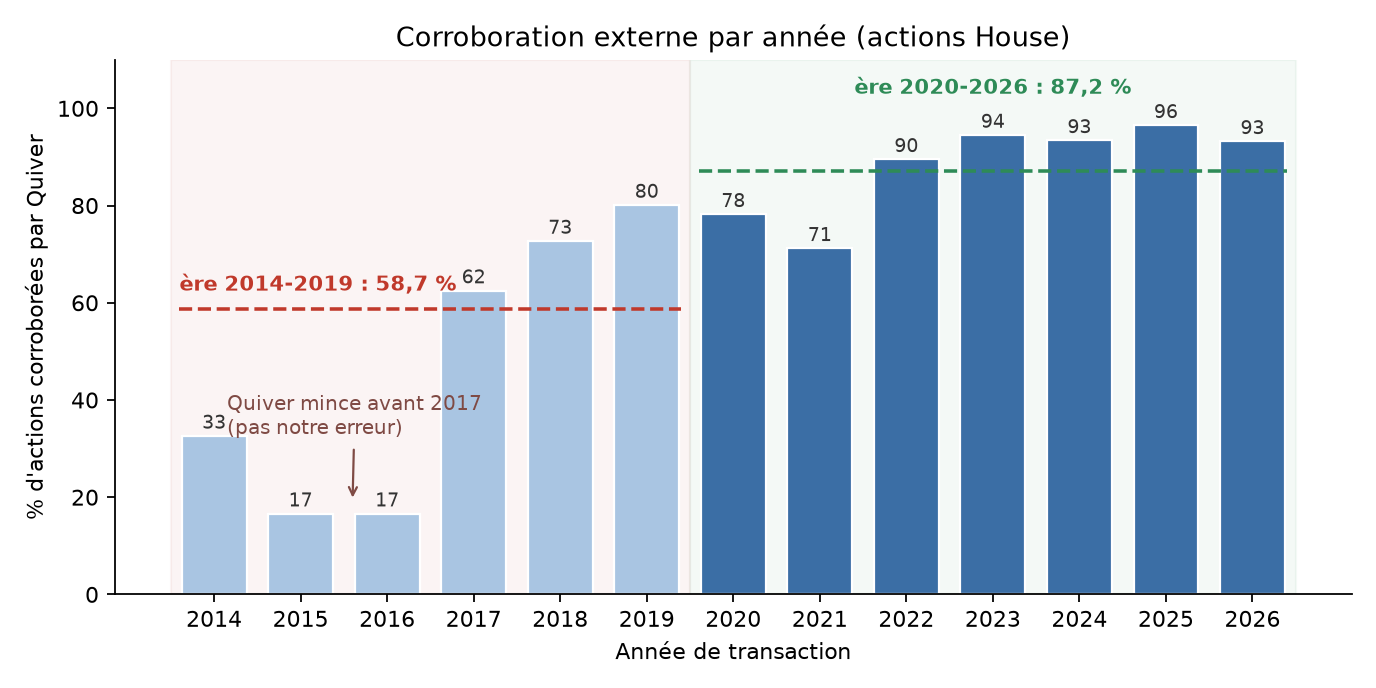
\includegraphics[width=\linewidth]{slides/fig_quiver_par_an.png}
    \end{column}
  \end{columns}
\end{frame}

% ───────────── S12 · Livrable + limites ─────────────
% Chiffres : §7 (134 464×36, entonnoir) ; 372 membres + 56 % OCR (CSV backtest) ;
% 582 manuscrits (§1) ; corroboration pré-2017 (§6.2) ; midpoint (§4)
\begin{frame}{Le livrable — et ses limites assumées}
  \begin{columns}[T]
    \begin{column}{0.60\textwidth}
      \centering
      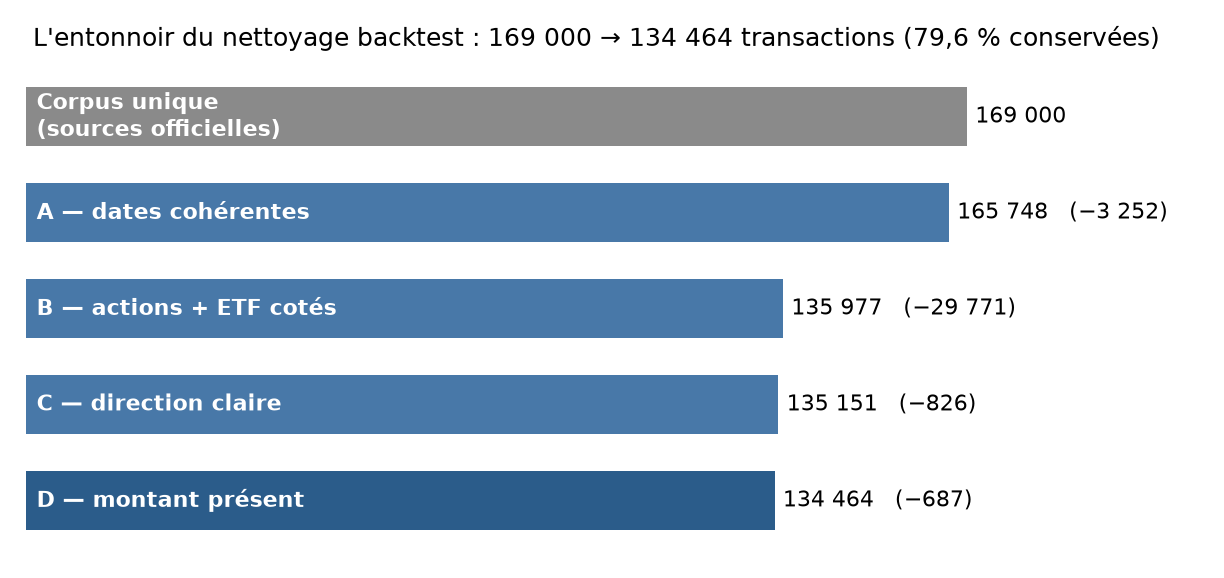
\includegraphics[width=\linewidth]{quality/entonnoir_backtest.png}
    \end{column}
    \begin{column}{0.38\textwidth}
      \colorbox{helec}{\parbox{0.96\linewidth}{\footnotesize\color{white}\centering\vspace{1mm}
        \texttt{\scriptsize transactions\_backtest\_2014\_2026.csv}\\[1mm]
        \textbf{134\,464 lignes × 36 colonnes}\\
        372 membres · 57\,\% issu d'OCR\\
        traçable ligne à ligne (\texttt{doc\_id})\vspace{1mm}}}
      \vspace{3.5mm}

      {\footnotesize\textbf{Limites assumées}}\\[1mm]
      {\scriptsize
      \textcolor{alertred}{\textbf{·}} 582 PTR manuscrits écartés (règle rejouable)\\[0.8mm]
      \textcolor{alertred}{\textbf{·}} corroboration externe plus faible avant 2017\\[0.8mm]
      \textcolor{alertred}{\textbf{·}} montants = fourchettes (milieu), pas des prix}
    \end{column}
  \end{columns}
\end{frame}

% ───────────── Annexes ─────────────
\appendix

% Backup A : volumes par an × voie — fig générée depuis les FINAL (load_final, totaux contrôlés)
\begin{frame}{Annexe — volumes par année et par voie}
  \centering
  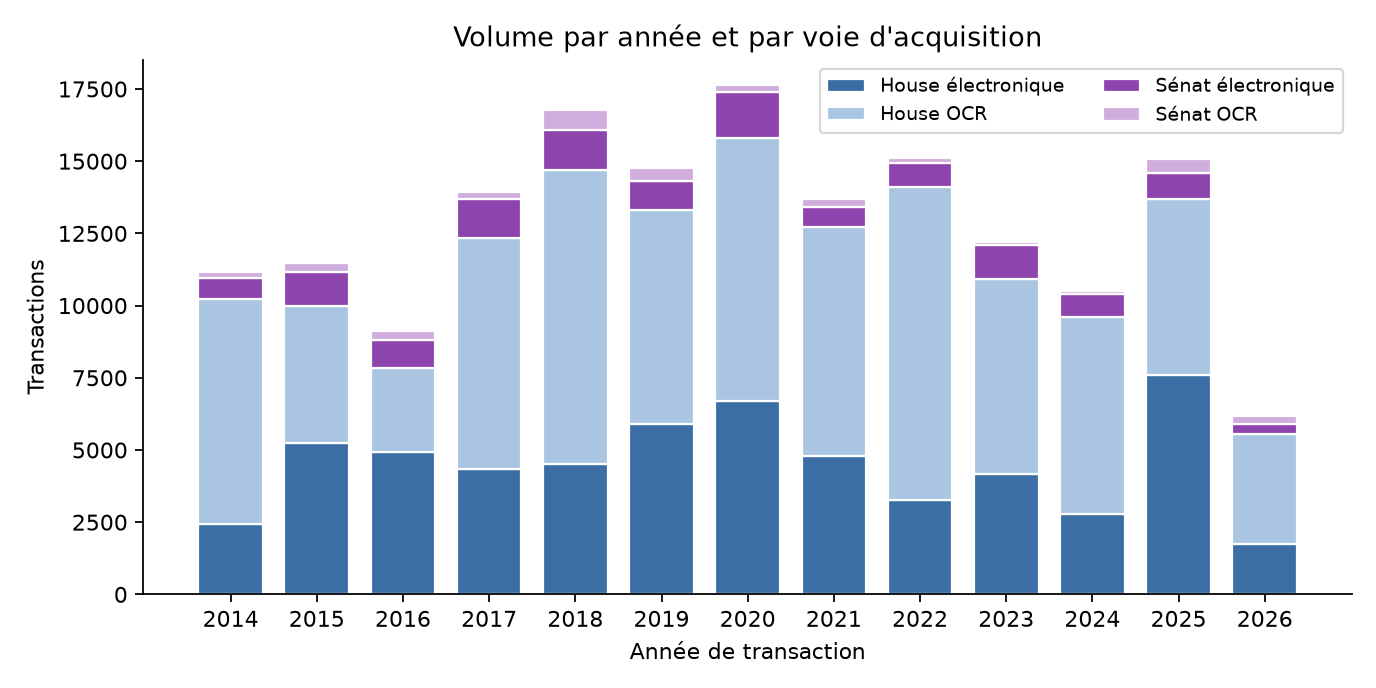
\includegraphics[width=0.86\textwidth]{slides/fig_par_an_voie.png}\\[1mm]
  {\scriptsize\color{black!60} totaux contrôlés = 169\,000 transactions uniques ;
   1\,381 transactions antérieures à 2014 (régularisations tardives) non tracées}
\end{frame}

% Backup B : les deux extrêmes en vrai (PDF réels du corpus)
\begin{frame}{Annexe — les deux extrêmes, en vrai}
  \centering
  \begin{minipage}[t]{0.44\textwidth}\centering
    \fcolorbox{helec}{white}{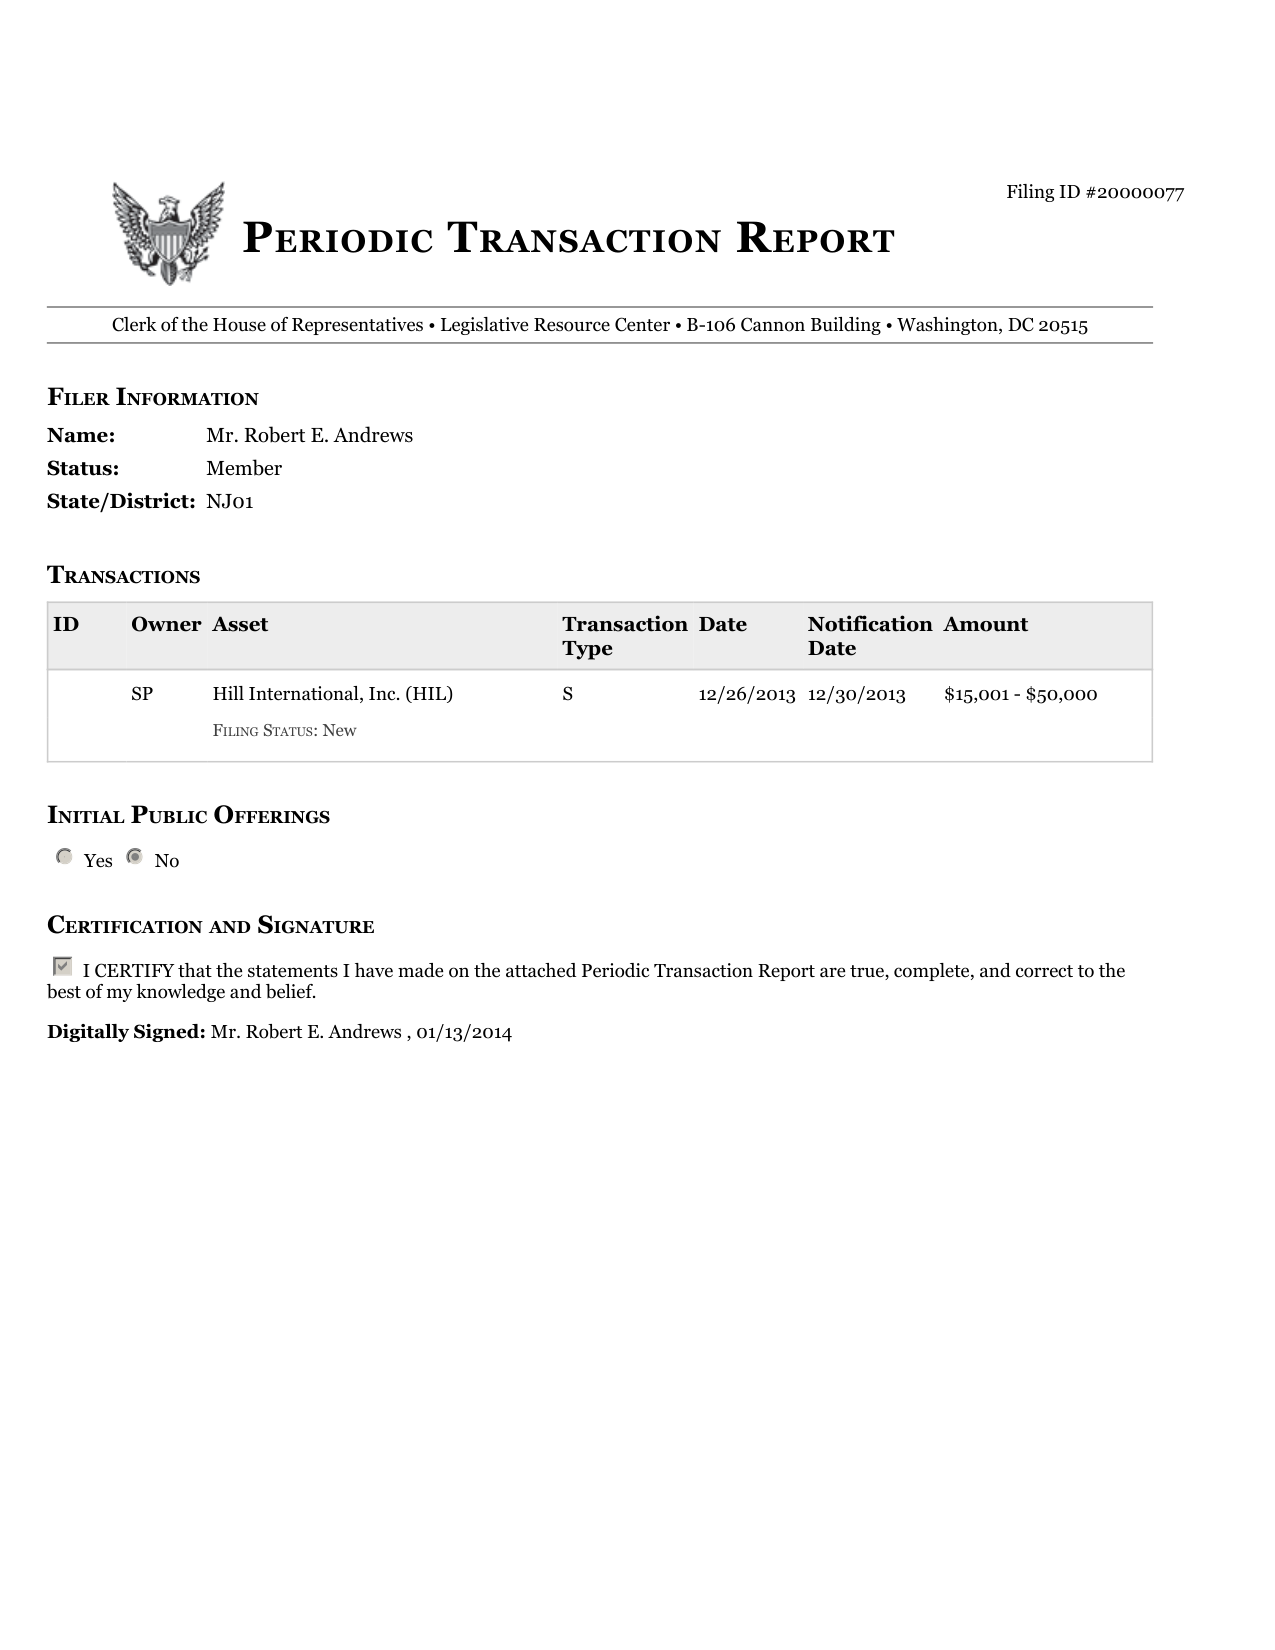
\includegraphics[height=52mm]{slides/fig_pdf_digital_2014.png}}\\[0.8mm]
    \badge{helec}{PTR électronique 2014 (doc 20000077)}\\[0.4mm]
    {\scriptsize ancien gabarit — d'où le double parseur}
  \end{minipage}\hspace{8mm}
  \begin{minipage}[t]{0.44\textwidth}\centering
    \fcolorbox{hocr}{white}{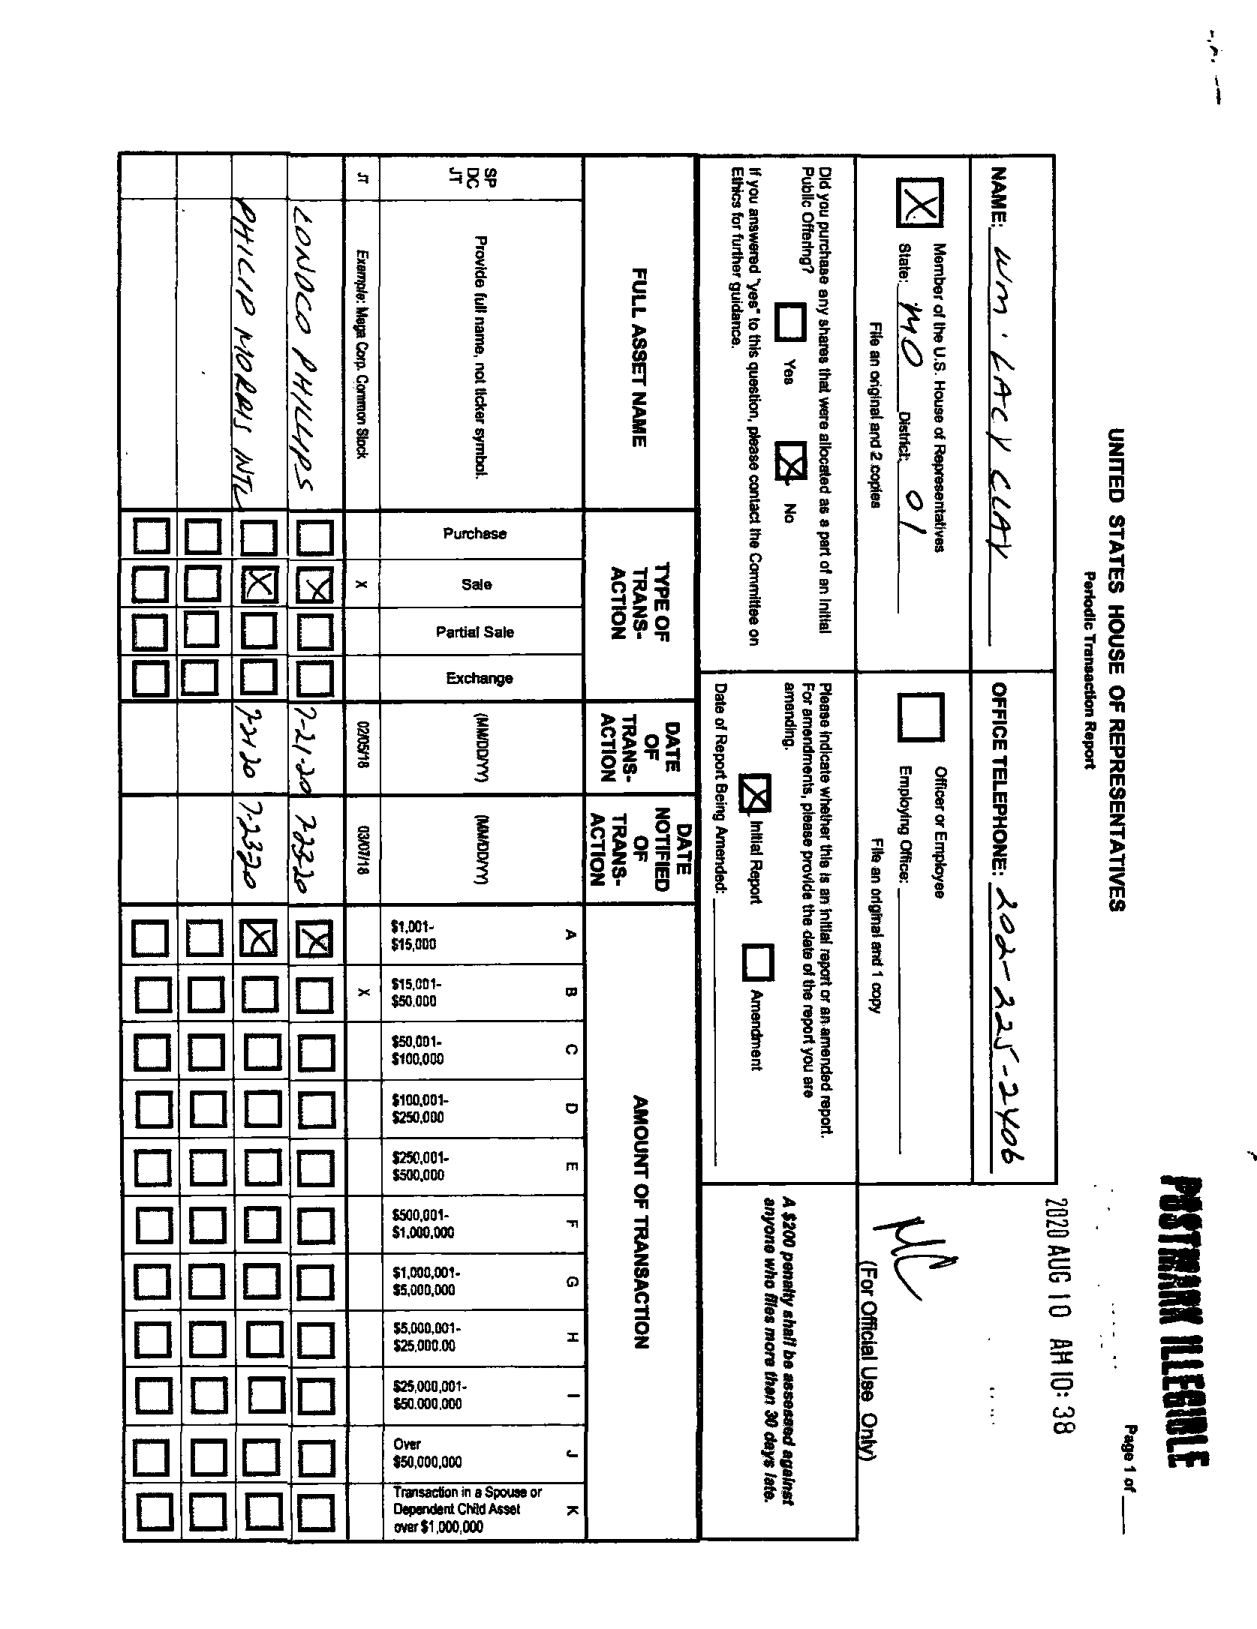
\includegraphics[height=52mm]{slides/fig_pdf_manuscrit_clay.png}}\\[0.8mm]
    \badgel{hocr}{PTR manuscrit 2020 (doc 8217474)}\\[0.4mm]
    {\scriptsize cursif, tourné, tampon « postmark illegible »}
  \end{minipage}
\end{frame}

\end{document}
